\documentclass{scrartcl}

\usepackage[svgnames,pdftex,dvipsnames]{xcolor}

\usepackage{tikz}
\usetikzlibrary{plotmarks}
\usetikzlibrary{decorations}
\usetikzlibrary{shapes}

\newcommand{\name}[1]{{\sc #1}}
\newcommand{\GrGen}{\name{GrGen}}
\newcommand{\grgennet}{\name{GrGen.NET}}
\newcommand{\libgr}{\name{libGr}}
\newcommand{\grshell}{\name{GrShell}}
\newcommand{\fujaba}{\name{Fujaba}}
\newcommand{\agg}{\name{AGG}}
\newcommand{\varrodb}{Varr{\'o}DB}
\newcommand{\progres}{\name{PROGRES}}

\begin{document}

\begin{figure} [bt]
	\centering
	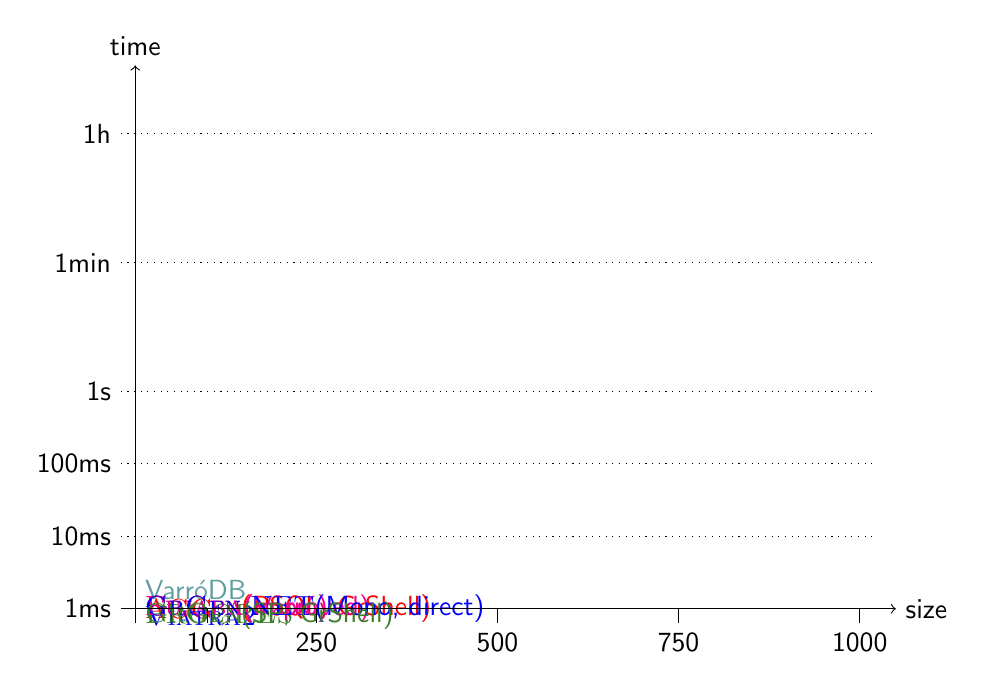
\begin{tikzpicture} [scale=0.92]
        \sf
		\draw[color=red] plot[mark=triangle*,mark options={color=red, rotate=180}]
			file{results/agg-Mutex.table} node[right] {\agg};
		\draw[color=CadetBlue] plot[mark=triangle*,mark options={color=black}]
			file{results/varrodb-Mutex_varro_scaled.table} node[above right] {\varrodb};
		\draw[color=OliveGreen] plot[mark=star, mark options={color=black}]
			file{results/progres-Mutex_varro_scaled.table} +(0,-0.07) node[right] {\progres};

        \draw[color=blue] plot[mark=*,mark options={color=black}]
			file{results/viatra2.table} +(0,-0.1) node[right] {{\sc Viatra2}};

		\draw[color=red] plot[mark=square, mark options={color=red}]
			file{results/psql-Mutex_opt.table} node[right] {\GrGen(PSQL, GrShell)};

        \draw[color=magenta] plot[mark=*,mark options={color=black}]
			file{results/fujaba-Mutex_varro_scaled.table} node[right] {\fujaba(Varr{\'o})};

        \draw[color=magenta] plot[mark=*,mark options={color=black}]
			file{results/mutex_fujaba_many_mo_fixed_10_100-1000.txt.table} node[right] {\fujaba(improved)};

		\draw[color=blue] plot[mark=square, mark options={color=blue}]
			file{results/mutex_mono_lgsp_small_10-1000.txt.table} node[right] {\grgennet(Mono, direct)};
%		\draw[color=blue] plot[mark=square, mark options={color=blue}]
%			file{results/fb-Mutex_opt6.table} node[right] {\GrGen(SP, GrShell)};

    	\draw[color=OliveGreen] plot[mark=square, mark options={color=OliveGreen}]
			file{results/grgenc_grshell_100-1000_toldtime_better.txt.table} +(0,-0.1) node[right] {\GrGen(SP, GrShell)};

		\draw[->] (-0.2,0) -- (10.5,0) node[right] {size};
		\draw[->] (0,-0.2) -- (0,7.5) node[above] {time};
		\draw[dotted] (-0.2,0) node[left] {1ms} -- (10.2,0);
		\draw[dotted] (-0.2,1) node[left] {10ms} -- (10.2,1);
		\draw[dotted] (-0.2,2) node[left] {100ms} -- (10.2,2);
		\draw[dotted] (-0.2,3) node[left] {1s} -- (10.2,3);
		\draw[dotted] (-0.2,4.77815125038364363252) node[left] {1min} -- (10.2,4.77815125038364363252);
		\draw[dotted] (-0.2,6.55630250076728726503) node[left] {1h} -- (10.2,6.55630250076728726503) ;
		\draw (1,-0.2)   node[below] {100}  -- (1,0);
		\draw (2.5,-0.2) node[below] {250}  -- (2.5,0);
		\draw (5,-0.2)   node[below] {500}  -- (5,0);
		\draw (7.5,-0.2) node[below] {750}  -- (7.5,0);
		\draw (10,-0.2) node[below]  {1000} -- (10,0);
	\end{tikzpicture}
	\caption{Running times of the STSmany benchmark for different graph rewrite systems}
	\label{fig:compareTools}
\end{figure}

\begin{figure} [phtb]
	\centering
	\begin{tikzpicture} [scale=1.15]
        \sf
		\draw[color=red] plot[mark=triangle*,mark options={color=red, rotate=180}]
			file{results/agg-Mutex.dtable} node[right] {\agg};
		\draw[color=CadetBlue] plot[mark=triangle*,mark options={color=black}]
			file{results/varrodb-Mutex_varro_scaled.dtable} +(0,0.2) node[right] {\varrodb};
		\draw[color=OliveGreen] plot[mark=star, mark options={color=black}]
			file{results/progres-Mutex_varro_scaled.dtable} +(0,-0.08) node[right] {\progres};

        \draw[color=blue] plot[mark=*,mark options={color=black}]
			file{results/viatra2.dtable} node[right] {{\sc Viatra2}};

		\draw[color=red] plot[mark=square, mark options={color=red}]
			file{results/psql-Mutex_opt.dtable} +(0,0.45) node[right] {\GrGen(PSQL, GrShell)};

        \draw[color=magenta] plot[mark=*,mark options={color=black}]
			file{results/mutex_fujaba_linux_many_mo_fixed_nolog4j_10-10000.txt.dtable} +(0,0.0) node[right] {\fujaba(improved)};

		\draw[color=OliveGreen] plot[mark=square, mark options={color=OliveGreen}]
			file{results/grgenc_grshell_10-1000000_toldtime.txt.dtable} +(-6.2,-3.6) node[right] {\GrGen(SP, GrShell)};
		\draw[color=blue] plot[mark=square, mark options={color=blue}]
			file{results/mutex_mono_lgsp_withjittime_10-1000000.txt.dtable} +(-3.4,-2) node[right] {\grgennet(Mono, direct)};

		\draw[->] (0.8,0) -- (12.5,0) node[right] {size};
		\draw[->] (1,-0.2) -- (1,7.5) node[above] {time};
		\draw[dotted] (0.8,0) node[left] {1ms} -- (12.2,0);
		\draw[dotted] (0.8,1) node[left] {10ms} -- (12.2,1);
		\draw[dotted] (0.8,2) node[left] {100ms} -- (12.2,2);
		\draw[dotted] (0.8,3) node[left] {1s} -- (12.2,3);
		\draw[dotted] (0.8,4.77815125038364363252) node[left] {1min} -- (12.2,4.77815125038364363252);
		\draw[dotted] (0.8,6.55630250076728726503) node[left] {1h} -- (12.2,6.55630250076728726503);
		\draw (2,-0.2)  node[below] {10}      -- (2,0);
		\draw (4,-0.2)  node[below] {100}     -- (4,0);
		\draw (6,-0.2)  node[below] {1000}    -- (6,0);
		\draw (8,-0.2)  node[below] {10000}   -- (8,0);
		\draw (10,-0.2) node[below] {100000}  -- (10,0);
		\draw (12,-0.2) node[below] {1000000} -- (12,0);
	\end{tikzpicture}
	\caption{Running times of the STSmany benchmark for different graph rewrite systems}
	\label{fig:compareToolsDoubleLog}
\end{figure}

\begin{figure} [phtb]
	\centering
	\begin{tikzpicture} [scale=1.15]	% 0.9
        \sf
		\draw[color=red] plot[mark=triangle*,mark options={color=red, rotate=180}]
			file{results/agg-Mutex.dtable} node[right] {\agg};
		\draw[color=CadetBlue] plot[mark=triangle*,mark options={color=black}]
			file{results/varrodb-Mutex_varro_scaled.dtable} +(0,0.2) node[right] {\varrodb};
		\draw[color=OliveGreen] plot[mark=star, mark options={color=black}]
			file{results/progres-Mutex_varro_scaled.dtable} +(0,-0.08) node[right] {\progres};

        \draw[color=blue] plot[mark=*,mark options={color=black}]
			file{results/viatra2.dtable} node[right] {{\sc Viatra2}};

        \draw[color=red] plot[mark=square, mark options={color=red}]
			file{results/psql-Mutex_opt.dtable} +(0,0.45) node[right] {\GrGen(PSQL, GrShell)};

        \draw[color=magenta] plot[mark=*,mark options={color=black}]
			file{results/mutex_fujaba_linux_many_mo_fixed_nolog4j_nojittime_10-10000.txt.dtable} +(0,0.0) node[right] {\fujaba(improved)};

		\draw[color=OliveGreen] plot[mark=square, mark options={color=OliveGreen}]
			file{results/grgenc_grshell_10-1000000_toldtime.txt.dtable} +(-6.2,-3.6) node[right] {\GrGen(SP, GrShell)};
		\draw[color=blue] plot[mark=square, mark options={color=blue}]
			file{results/mutex_mono_lgsp_nojittime_10-1000000.txt.dtable} +(-3.2,-2.3) node[right] {\grgennet(Mono, direct)};

		\draw[->] (0.8,0) -- (12.5,0) node[right] {size};
		\draw[->] (1,-0.2) -- (1,7.5) node[above] {time};
		\draw[dotted] (0.8,0) node[left] {1ms} -- (12.2,0);
		\draw[dotted] (0.8,1) node[left] {10ms} -- (12.2,1);
		\draw[dotted] (0.8,2) node[left] {100ms} -- (12.2,2);
		\draw[dotted] (0.8,3) node[left] {1s} -- (12.2,3);
		\draw[dotted] (0.8,4.77815125038364363252) node[left] {1min} -- (12.2,4.77815125038364363252);
		\draw[dotted] (0.8,6.55630250076728726503) node[left] {1h} -- (12.2,6.55630250076728726503);
		\draw (2,-0.2)  node[below] {10}      -- (2,0);
		\draw (4,-0.2)  node[below] {100}     -- (4,0);
		\draw (6,-0.2)  node[below] {1000}    -- (6,0);
		\draw (8,-0.2)  node[below] {10000}   -- (8,0);
		\draw (10,-0.2) node[below] {100000}  -- (10,0);
		\draw (12,-0.2) node[below] {1000000} -- (12,0);
	\end{tikzpicture}
	\caption{Running times of the STSmany benchmark for different graph rewrite systems with a warm-up run (n=1000) for \fujaba\ and \grgennet\ to reduce JIT overhead}
	\label{fig:compareToolsDoubleLogNOJIT}
\end{figure}

\end{document}
